% ======================================================================
%  Why Most Fermion-to-Qubit Encoding Trees Don't Work
%  —  An Explainer for the Star-Tree Theorem
% ======================================================================
%
%  Target audience: researchers familiar with fermion-to-qubit encodings
%  who want an accessible account of the star-tree limitation and how
%  F# symbolic computation uncovered it.
%
%  Compile: latexmk -pdf explainer.tex
% ======================================================================
\documentclass[11pt,a4paper]{article}

\usepackage[utf8]{inputenc}
\usepackage[T1]{fontenc}
\usepackage{lmodern}
\usepackage{amsmath,amssymb,amsthm}
\usepackage{booktabs}
\usepackage{hyperref}
\usepackage{xcolor}
\usepackage{tikz}
\usepackage{braket}
\usepackage{mathtools}
\usepackage{cleveref}
\usepackage{fancyvrb}
\usepackage{tcolorbox}
\usepackage[margin=2.5cm]{geometry}
\usepackage{enumitem}
\usepackage{caption}

\usetikzlibrary{trees,positioning,arrows.meta,calc,decorations.pathmorphing,
  backgrounds,fit,shapes.geometric}

\hypersetup{
  colorlinks=true,
  linkcolor=blue!70!black,
  citecolor=green!50!black,
  urlcolor=blue!60!black,
}

% --- Custom commands ------------------------------------------------
\newcommand{\ad}[1]{a_{#1}^{\dagger}}
\newcommand{\an}[1]{a_{#1}^{\vphantom{\dagger}}}
\newcommand{\acomm}[2]{\{#1,\,#2\}}
\newcommand{\Uset}[1]{U(#1)}
\newcommand{\Pset}[1]{P(#1)}
\newcommand{\Occ}[1]{\mathrm{Occ}(#1)}

\newtheorem{theorem}{Theorem}
\newtheorem{corollary}[theorem]{Corollary}
\theoremstyle{definition}
\newtheorem{definition}[theorem]{Definition}

% Code highlighting box
\tcbuselibrary{listings,skins}
\newtcblisting{fsharpcode}[1][]{%
  colback=gray!5,
  colframe=blue!50!black,
  fonttitle=\bfseries\ttfamily,
  listing only,
  listing options={
    language=ML,
    basicstyle=\small\ttfamily,
    keywordstyle=\color{blue!70!black}\bfseries,
    commentstyle=\color{green!50!black}\itshape,
    stringstyle=\color{red!60!black},
    showstringspaces=false,
    columns=flexible,
    morekeywords={let,type,match,with,fun,module,open,namespace,if,then,else,%
      Set,int,List,map,fold,filter},
  },
  title={#1},
}

% Callout box for key insights
\newtcolorbox{keyinsight}[1][]{%
  colback=yellow!8,
  colframe=orange!70!black,
  fonttitle=\bfseries,
  title={Key Insight},
  #1
}

% Callout box for "what was believed"
\newtcolorbox{believed}[1][]{%
  colback=blue!5,
  colframe=blue!50!black,
  fonttitle=\bfseries,
  title={What Was Believed},
  #1
}

% Callout box for "what we found"
\newtcolorbox{found}[1][]{%
  colback=red!5,
  colframe=red!50!black,
  fonttitle=\bfseries,
  title={What We Found},
  #1
}

%%====================================================================
\begin{document}

\title{\bfseries Why Most Fermion-to-Qubit\\Encoding Trees Don't Work\\[6pt]
  \large An Explainer for the Star-Tree Theorem}

\author{John S Azariah\\
  \small Centre for Quantum Software and Information,\\
  \small School of Computer Science,\\
  \small Faculty of Engineering \& Information Technology,\\
  \small University of Technology Sydney, NSW 2007, Australia\\
  \small\texttt{john.azariah@student.uts.edu.au}\\
  \small ORCID: \href{https://orcid.org/0009-0007-9870-1970}{0009-0007-9870-1970}}

\date{February 2026}

\maketitle

\begin{abstract}
The Seeley--Richard--Love (SRL) index-set framework is widely cited as
providing a unified, parameterized treatment of fermion-to-qubit
encodings.  We explain a surprising structural limitation: the generic
SRL construction satisfies the canonical anticommutation relations
\emph{if and only if} the underlying tree is a star (depth~$\le 1$).
This means only relabelled Jordan--Wigner and Parity encodings emerge
from the generic recipe --- all deeper trees fail.  We walk through the
proof visually, explain how F\# symbolic computation uncovered the
result, and discuss what it means for the field.
\end{abstract}

\tableofcontents
\vspace{1em}

%%====================================================================
\section{The Story So Far}
\label{sec:story}

%%--------------------------------------------------------------------
\subsection{The encoding problem}

Quantum simulation of chemistry and materials requires mapping
fermionic operators (creation and annihilation operators
$\ad{j}$, $\an{j}$) to qubit operators (Pauli strings).  The
challenge is that fermions anticommute:
\begin{equation}
  \acomm{\an{i}}{\ad{j}} = \delta_{ij}, \qquad
  \acomm{\an{i}}{\an{j}} = 0, \qquad
  \acomm{\ad{i}}{\ad{j}} = 0,
  \label{eq:car}
\end{equation}
while Pauli operators either commute or anticommute depending on their
structure.  Getting this right is the whole game.

\begin{figure}[h]
\centering
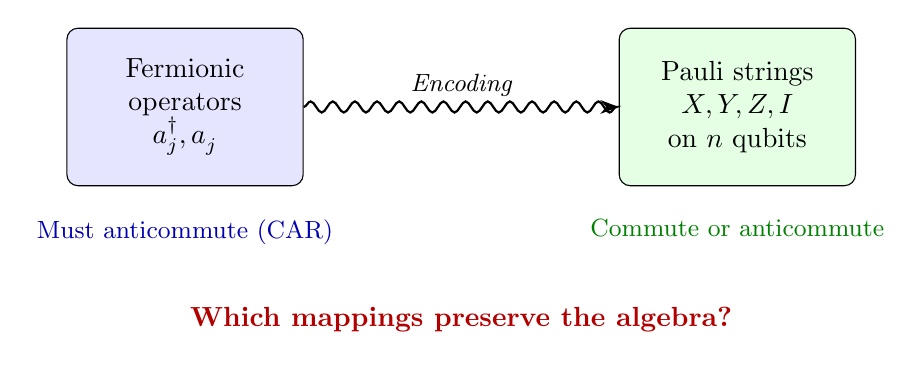
\begin{tikzpicture}[>=Stealth, node distance=3cm]
  % Left: Fermion world
  \node[draw, rounded corners, fill=blue!10, minimum width=3cm,
        minimum height=2cm, align=center] (ferm)
    {Fermionic\\operators\\$\ad{j}, \an{j}$};

  % Right: Qubit world
  \node[draw, rounded corners, fill=green!10, minimum width=3cm,
        minimum height=2cm, align=center, right=4cm of ferm] (qubit)
    {Pauli strings\\$X, Y, Z, I$\\on $n$ qubits};

  % Arrow
  \draw[->, thick, decorate, decoration={snake, amplitude=2pt, segment length=8pt}]
    (ferm) -- node[above, font=\small\itshape] {Encoding} (qubit);

  % Constraint
  \node[below=0.3cm of ferm, font=\small, text=blue!70!black]
    (lbl-left) {Must anticommute (CAR)};
  \node[below=0.3cm of qubit, font=\small, text=green!50!black]
    (lbl-right) {Commute or anticommute};

  % The question
  \node[below=0.6cm of $(lbl-left.south)!0.5!(lbl-right.south)$,
        font=\bfseries, text=red!70!black]
    {Which mappings preserve the algebra?};
\end{tikzpicture}
\caption{The fermion-to-qubit encoding problem: find a map that
preserves anticommutation.}
\label{fig:encoding-problem}
\end{figure}

%%--------------------------------------------------------------------
\subsection{Three well-known encodings}

Three encodings dominate the literature:

\begin{center}
\begin{tabular}{@{}llll@{}}
\toprule
Encoding & Year & Pauli weight & Key idea \\
\midrule
Jordan--Wigner (JW) & 1928 & $O(n)$ & Parity string \\
Bravyi--Kitaev (BK) & 2002 & $O(\log n)$ & Fenwick tree \\
Parity & 2012 & $O(n)$ & Complement of JW \\
\bottomrule
\end{tabular}
\end{center}

Each was discovered independently, with its own derivation and
correctness proof.

%%--------------------------------------------------------------------
\subsection{The SRL ``unification'' (2012)}

\begin{believed}
Seeley, Richard, and Love showed that JW, BK, and Parity are all
special cases of a \textbf{single parameterized framework}.  You
choose three set-valued functions --- $U(j)$, $P(j)$, $\Occ{j}$ ---
and a universal algorithm builds the encoding automatically.

\medskip

The natural conclusion, adopted across the field: \textbf{the framework
is general}.  Any valid choice of index sets should give a valid
encoding.  Trees provide a systematic way to generate such sets.
\end{believed}

The SRL paper presents a single recipe for building Majorana operators
from any triple of index-set functions.  Different choices yield
different encodings:

\begin{figure}[h]
\centering
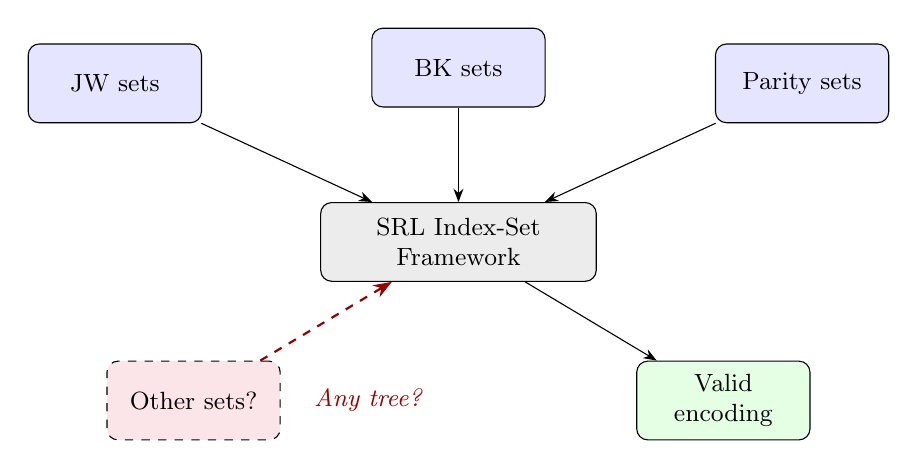
\begin{tikzpicture}[
  box/.style={draw, rounded corners, minimum width=2.2cm,
              minimum height=1cm, align=center, font=\small},
  >=Stealth
]
  % Central box
  \node[box, fill=gray!15, minimum width=3.5cm] (srl)
    {SRL Index-Set\\Framework};

  % Inputs
  \node[box, fill=blue!10, above left=1cm and 1.5cm of srl] (jw)
    {JW sets};
  \node[box, fill=blue!10, above=1.2cm of srl] (bk)
    {BK sets};
  \node[box, fill=blue!10, above right=1cm and 1.5cm of srl] (par)
    {Parity sets};
  \node[box, fill=blue!10!red!10, below left=1cm and 0.5cm of srl,
        dashed] (other)
    {Other sets?};

  % Output
  \node[box, fill=green!10, below right=1cm and 0.5cm of srl] (enc)
    {Valid\\encoding};

  % Arrows
  \draw[->] (jw) -- (srl);
  \draw[->] (bk) -- (srl);
  \draw[->] (par) -- (srl);
  \draw[->, dashed, thick, red!60!black] (other) -- (srl);
  \draw[->] (srl) -- (enc);

  % Question
  \node[right=0.3cm of other, font=\small\itshape, text=red!60!black]
    {Any tree?};
\end{tikzpicture}
\caption{The SRL vision: a universal framework parameterized by index
sets.  The question: does every tree produce valid sets?}
\label{fig:srl-vision}
\end{figure}

%%====================================================================
\section{How the Index-Set Method Works (Construction A)}
\label{sec:construction-a}

Before we can understand \emph{why} the SRL framework fails for deep
trees, we need to understand \emph{how} it works.  This is what we
call Construction~A: the generic index-set derivation.

%%--------------------------------------------------------------------
\subsection{The three index sets}

For each fermionic mode~$j$ (from $0$ to $n{-}1$), Construction~A
specifies three sets of qubit indices:

\begin{center}
\begin{tabular}{@{}lp{8cm}@{}}
\toprule
\textbf{Set} & \textbf{Meaning} \\
\midrule
$U(j)$ --- Update &
  Which \emph{other} qubits must be flipped when mode~$j$ changes
  occupation.  These are the qubits that store partial sums
  involving mode~$j$. \\
$P(j)$ --- Parity &
  Which qubits collectively encode the running parity of modes
  below~$j$.  Needed to enforce anticommutation. \\
$\Occ{j}$ --- Occupation &
  Which qubits collectively determine whether mode~$j$ is filled
  or empty. \\
\bottomrule
\end{tabular}
\end{center}

%%--------------------------------------------------------------------
\subsection{The encoding algorithm}

Given these three sets, the Majorana operators for mode~$j$ are built
by the formulas:
\begin{align}
  c_j &= X_{\{j\} \cup U(j)} \;\cdot\; Z_{P(j)},
  \label{eq:cj-consA} \\[4pt]
  d_j &= Y_j \;\cdot\; X_{U(j)} \;\cdot\;
    Z_{(P(j)\,\triangle\,\Occ{j})\,\setminus\,\{j\}},
  \label{eq:dj-consA}
\end{align}
where $X_S$ means ``put $X$ on every qubit in set $S$, identity
elsewhere,'' and $\triangle$ is the symmetric difference ($A
\triangle B$ = elements in $A$ or $B$ but not both).

In words:
\begin{itemize}
  \item $c_j$: put $X$ on qubit~$j$ and all its update qubits;
    put $Z$ on all its parity qubits.
  \item $d_j$: put $Y$ on qubit~$j$; put $X$ on its update qubits;
    put $Z$ on the ``leftover'' qubits from the symmetric difference
    of parity and occupation (minus~$j$ itself).
\end{itemize}

%%--------------------------------------------------------------------
\subsection{Deriving sets from a tree}

The SRL framework becomes a tree-based method when you derive the
three sets from a labelled rooted tree $T$.  The recipe is:
\begin{align*}
  U(j) &= \text{ancestors of } j \text{ in } T, \\
  P(j) &= \text{remainder}(j) \cup \text{children}(j), \\
  \Occ{j} &= \text{descendants}(j) \cup \{j\},
\end{align*}
where $\text{remainder}(j)$ collects children of ancestors of $j$
that have index~$< j$ and are not themselves ancestors of~$j$.

This always produces well-formed sets and yields Pauli strings of
the correct width.  The question is whether the resulting operators
satisfy the CAR.

%%--------------------------------------------------------------------
\subsection{Worked example: Jordan--Wigner as a star tree}

Consider $n = 4$ modes with the star tree rooted at node~3:

\begin{figure}[h]
\centering
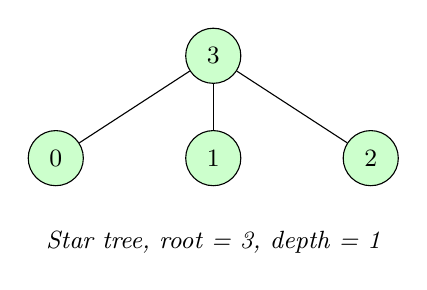
\begin{tikzpicture}[
  treeNode/.style={circle, draw, minimum size=0.7cm, inner sep=0pt,
                   font=\small, fill=green!20},
  >=Stealth
]
  \node[treeNode] (r) at (0,0) {3};
  \node[treeNode] (a) at (-2,-1.3) {0};
  \node[treeNode] (b) at (0,-1.3) {1};
  \node[treeNode] (c) at (2,-1.3) {2};
  \draw (r) -- (a);
  \draw (r) -- (b);
  \draw (r) -- (c);
  \node[below=0.3cm, font=\small\itshape] at (0,-1.8)
    {Star tree, root = 3, depth = 1};
\end{tikzpicture}
\caption{A star tree on 4 nodes.  Every non-root node is a direct
child of the root.}
\label{fig:star-example}
\end{figure}

Deriving sets from this tree:

\begin{center}
\begin{tabular}{@{}cccc@{}}
\toprule
Mode $j$ & $U(j)$ & $P(j)$ & $\Occ{j}$ \\
\midrule
0 & $\{3\}$ & $\emptyset$ & $\{0\}$ \\
1 & $\{3\}$ & $\{0\}$ & $\{1\}$ \\
2 & $\{3\}$ & $\{0, 1\}$ & $\{2\}$ \\
3 & $\emptyset$ & $\{0, 1, 2\}$ & $\{0, 1, 2, 3\}$ \\
\bottomrule
\end{tabular}
\end{center}

Applying the formulas for mode~1:
\[
  c_1 = X_{\{1,3\}} \cdot Z_{\{0\}}
      = Z \otimes X \otimes I \otimes X.
\]
This is exactly the Jordan--Wigner Majorana operator for mode~1
(up to qubit ordering).  The update set $\{3\}$ propagates the change
to the root; the parity set $\{0\}$ tracks the running parity.

\begin{keyinsight}
For star trees, the sets are simple: $U(j) = \{\text{root}\}$,
$P(j) = \{\text{lower siblings}\}$, $\Occ{j} = \{j\}$.  No overlaps,
no cancellations, no problems.  This produces relabelled JW and
Parity encodings.
\end{keyinsight}

%%--------------------------------------------------------------------
\subsection{What goes wrong for deeper trees}

Now consider a chain tree on the same 4 nodes: $3 \to 2 \to 1 \to 0$.

\begin{center}
\begin{tabular}{@{}cccc@{}}
\toprule
Mode $j$ & $U(j)$ & $P(j)$ & $\Occ{j}$ \\
\midrule
0 & $\{1, 2, 3\}$ & $\emptyset$ & $\{0\}$ \\
1 & $\{2, 3\}$ & $\{0\}$ & $\{0, 1\}$ \\
2 & $\{3\}$ & $\{0, 1\}$ & $\{0, 1, 2\}$ \\
3 & $\emptyset$ & $\{0, 1, 2\}$ & $\{0, 1, 2, 3\}$ \\
\bottomrule
\end{tabular}
\end{center}

Look at mode~2: $P(2) = \{0, 1\}$ and $\Occ{2} = \{0, 1, 2\}$.  The
symmetric difference is $P(2) \triangle \Occ{2} = \{2\}$ --- nodes
$0$ and $1$ appear in \emph{both} sets and cancel out.  This is the
cancellation mechanism that produces identity where there should be
non-identity operators, leading to even anticommutation counts and
CAR violations.

%%====================================================================
\section{What We Found: The Star-Tree Theorem}
\label{sec:theorem}

\begin{found}
The generic SRL construction satisfies the CAR \textbf{if and only if}
the tree has depth~$\le 1$ (a ``star'').

\medskip

This means \textbf{only JW, Parity, and their relabellings} emerge
from the generic recipe.  All other trees --- binary, ternary, Fenwick,
arbitrary --- silently produce incorrect encodings.
\end{found}

\begin{theorem}[Star-tree constraint]
\label{thm:star-tree}
Let $T$ be a labelled rooted tree on $[n]$, and derive index sets via
the standard tree-to-sets recipe.  The resulting Majorana operators
satisfy the CAR if and only if $T$ is a star (depth~$\le 1$).
\end{theorem}

\begin{figure}[h]
\centering
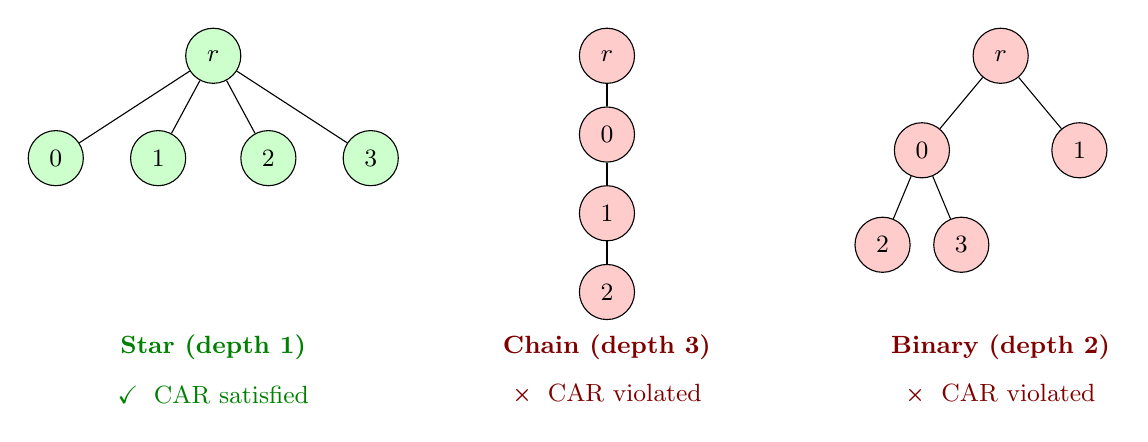
\begin{tikzpicture}[
  treeNode/.style={circle, draw, minimum size=0.7cm, inner sep=0pt,
                   font=\small},
  validTree/.style={fill=green!20},
  invalidTree/.style={fill=red!20},
  >=Stealth
]
  % === Star tree (valid) ===
  \begin{scope}[xshift=-5cm]
    \node[treeNode, validTree] (sr) at (0,0) {$r$};
    \node[treeNode, validTree] (s0) at (-2,-1.3) {$0$};
    \node[treeNode, validTree] (s1) at (-0.7,-1.3) {$1$};
    \node[treeNode, validTree] (s2) at (0.7,-1.3) {$2$};
    \node[treeNode, validTree] (s3) at (2,-1.3) {$3$};
    \draw (sr) -- (s0);
    \draw (sr) -- (s1);
    \draw (sr) -- (s2);
    \draw (sr) -- (s3);
    % Labels at common baseline
    \node[font=\small\bfseries, text=green!50!black] at (0,-3.7)
      {Star (depth 1)};
    \node[font=\small, text=green!50!black] at (0,-4.3)
      {\checkmark\; CAR satisfied};
  \end{scope}

  % === Linear chain (invalid) ===
  \begin{scope}[xshift=0cm]
    \node[treeNode, invalidTree] (lr) at (0,0) {$r$};
    \node[treeNode, invalidTree] (l0) at (0,-1) {$0$};
    \node[treeNode, invalidTree] (l1) at (0,-2) {$1$};
    \node[treeNode, invalidTree] (l2) at (0,-3) {$2$};
    \draw (lr) -- (l0) -- (l1) -- (l2);
    % Labels at common baseline
    \node[font=\small\bfseries, text=red!50!black] at (0,-3.7)
      {Chain (depth 3)};
    \node[font=\small, text=red!50!black] at (0,-4.3)
      {\texttimes\; CAR violated};
  \end{scope}

  % === Binary tree (invalid) ===
  \begin{scope}[xshift=5cm]
    \node[treeNode, invalidTree] (br) at (0,0) {$r$};
    \node[treeNode, invalidTree] (b0) at (-1,-1.2) {$0$};
    \node[treeNode, invalidTree] (b1) at (1,-1.2) {$1$};
    \node[treeNode, invalidTree] (b2) at (-1.5,-2.4) {$2$};
    \node[treeNode, invalidTree] (b3) at (-0.5,-2.4) {$3$};
    \draw (br) -- (b0) -- (b2);
    \draw (b0) -- (b3);
    \draw (br) -- (b1);
    % Labels at common baseline
    \node[font=\small\bfseries, text=red!50!black] at (0,-3.7)
      {Binary (depth 2)};
    \node[font=\small, text=red!50!black] at (0,-4.3)
      {\texttimes\; CAR violated};
  \end{scope}
\end{tikzpicture}
\caption{Only star trees (left) produce valid encodings via the SRL
generic construction.  Any tree with a grandchild --- chain (center),
binary (right), ternary, etc.\ --- fails.}
\label{fig:star-vs-deep}
\end{figure}

\subsection{``But wait --- the Bravyi--Kitaev encoding uses a deep tree!''}

Yes!  The BK encoding uses the Fenwick tree (depth $\sim \log_2 n$).
But it works not because of the \emph{generic} SRL construction ---
it works because its index sets are hand-derived using Fenwick-tree
bit-manipulation formulas that are \emph{specific} to that one tree
structure.  The SRL paper conflates two different things:

\begin{enumerate}
  \item A \textbf{generic algorithm} (plug in sets, get Majorana
    operators) --- this is what we call ``Construction~A''.
  \item A \textbf{hand-derived scheme} for the Fenwick tree
    (bit-masking formulas) --- this is what we call ``Construction~F''.
\end{enumerate}

Construction~F happens to produce results expressible as index sets,
but it is not an instance of the generic derivation process.

%%====================================================================
\section{The Proof, Visually}
\label{sec:proof}

The proof has two directions:

\begin{enumerate}
  \item \textbf{Stars work} (sufficiency) --- straightforward
    verification.
  \item \textbf{Only stars work} (necessity) --- the interesting
    direction.
\end{enumerate}

We focus on the necessity proof, which identifies the exact failure
mechanism.

%%--------------------------------------------------------------------
\subsection{The setup: a grandparent--parent--child path}

If a tree has depth $\ge 2$, there is guaranteed to be a path of three
vertices: grandparent $w$, parent $u$, child $v$.  We show that this
path causes the operators $d_w$ and $c_v$ to commute (even
anticommutation count), violating the CAR requirement
$\acomm{c_i}{d_j} = 0$.

The Majorana formulas from the SRL generic construction are:
\begin{align}
  c_v &= X_{\{v\} \cup U(v)} \cdot Z_{P(v)},
  \label{eq:cv} \\[4pt]
  d_w &= Y_w \cdot X_{U(w)} \cdot
    Z_{(P(w) \,\triangle\, \Occ{w}) \setminus \{w\}}.
  \label{eq:dw}
\end{align}

%%--------------------------------------------------------------------
\subsection{Step by step: what happens at each position}

\begin{figure}[h]
\centering
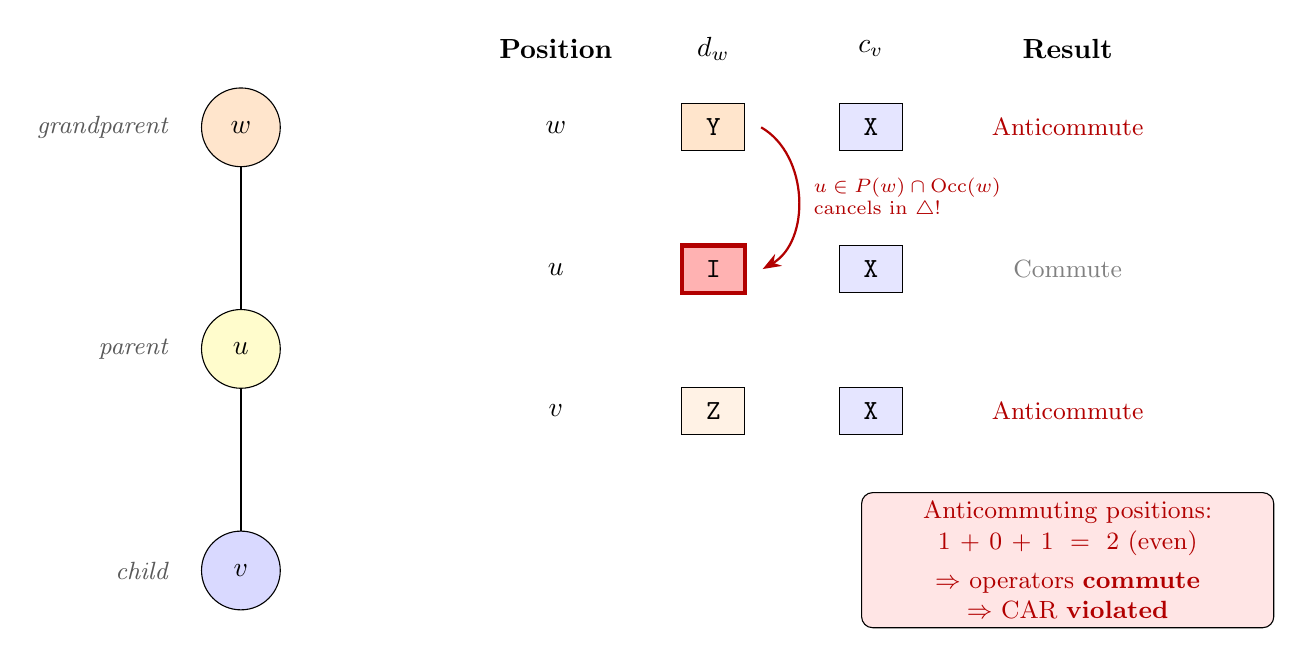
\begin{tikzpicture}[
  treeNode/.style={circle, draw, minimum size=1cm, inner sep=0pt,
                   font=\normalsize},
  pauliBox/.style={draw, minimum width=0.8cm, minimum height=0.6cm,
                   font=\normalsize\bfseries\ttfamily, inner sep=2pt},
  annot/.style={font=\small\itshape, text=gray!70!black},
  >=Stealth,
  node distance=2cm
]
  % Tree (shifted left to make room)
  \node[treeNode, fill=orange!20] (w) at (-1,0) {$w$};
  \node[treeNode, fill=yellow!20, below=1.8cm of w] (u) {$u$};
  \node[treeNode, fill=blue!15, below=1.8cm of u] (v) {$v$};
  \draw[thick] (w) -- (u) -- (v);

  % Annotations on the left
  \node[left=0.3cm of w, annot] {grandparent};
  \node[left=0.3cm of u, annot] {parent};
  \node[left=0.3cm of v, annot] {child};

  % Column headers — placed at fixed x positions
  \node[font=\bfseries] (hpos) at (3,1) {Position};
  \node[font=\bfseries] (hdw) at (5,1) {$d_w$};
  \node[font=\bfseries] (hcv) at (7,1) {$c_v$};
  \node[font=\bfseries] (hres) at (9.5,1) {Result};

  % Row w (grandparent) — aligned to tree node y
  \node at (3,0) (pos_w) {$w$};
  \node[pauliBox, fill=orange!20] at (5,0) (dw_w) {Y};
  \node[pauliBox, fill=blue!10] at (7,0) (cv_w) {X};
  \node[font=\small, text=red!70!black] at (9.5,0) (res_w) {Anticommute};

  % Row u (parent) — THE KEY
  \node at (3,-1.8) (pos_u) {$u$};
  \node[pauliBox, fill=red!30, draw=red!70!black, line width=1.5pt]
    at (5,-1.8) (dw_u) {I};
  \node[pauliBox, fill=blue!10] at (7,-1.8) (cv_u) {X};
  \node[font=\small, text=gray] at (9.5,-1.8) (res_u) {Commute};

  % Row v (child)
  \node at (3,-3.6) (pos_v) {$v$};
  \node[pauliBox, fill=orange!10] at (5,-3.6) (dw_v) {Z};
  \node[pauliBox, fill=blue!10] at (7,-3.6) (cv_v) {X};
  \node[font=\small, text=red!70!black] at (9.5,-3.6) (res_v) {Anticommute};

  % Cancellation annotation — routed to the right of dw column
  \draw[<-, thick, red!70!black] ([xshift=0.2cm]dw_u.east)
    to[out=30, in=-30]
    node[right, font=\scriptsize, text=red!70!black, align=left,
         xshift=2pt]
      {$u \in P(w) \cap \Occ{w}$\\cancels in $\triangle$!}
    ([xshift=0.2cm]dw_w.east);

  % Result box
  \node[below=0.8cm of res_v, draw, rounded corners, fill=red!10,
        text=red!70!black, font=\small, align=center, text width=5cm]
    {Anticommuting positions: $1 + 0 + 1 = 2$ (even)\\[3pt]
     $\Rightarrow$ operators \textbf{commute}\\
     $\Rightarrow$ CAR \textbf{violated}};
\end{tikzpicture}
\caption{The failure mechanism.  At the parent position $u$, the
symmetric-difference cancellation ($u$ is in \emph{both} $P(w)$ and
$\Occ{w}$, so it cancels out) assigns identity to $d_w$, while $c_v$
has $X$ there (since $u$ is an ancestor of $v$).  The resulting even
count of anticommuting positions means the operators commute instead
of anticommuting.}
\label{fig:failure-mechanism}
\end{figure}

Let's trace through each position on the $w \to u \to v$ path:

\begin{description}[leftmargin=2cm, font=\bfseries]
  \item[Position $w$:]
    $d_w$ has $Y$ (it's the ``home'' position, first term).
    $c_v$ has $X$ (since $w$ is an ancestor of $v$, so $w \in U(v)$).
    $Y$ and $X$ \textbf{anticommute}.

  \item[Position $u$:]
    This is the critical position.

    $c_v$ has $X$ at $u$, because $u$ is an ancestor of $v$.

    What about $d_w$?  Node $u$ is a child of $w$, so
    $u \in P(w)$.  And $u$ is a descendant of $w$, so
    $u \in \Occ{w}$.  The formula for $d_w$ uses
    $P(w) \,\triangle\, \Occ{w}$ --- positions in $P$ XOR $\Occ$.
    Since $u$ is in \emph{both}, it cancels out!  So $d_w$ has
    $I$ (identity) at position $u$.

    $I$ and $X$ \textbf{commute}.

  \item[Position $v$:]
    $d_w$ has $Z$ at $v$ (node $v$ is a descendant of $w$ so
    $v \in \Occ{w}$, but $v$ is not a child of $w$ so
    $v \notin P(w)$; it survives in the symmetric difference).
    $c_v$ has $X$ (home position).
    $Z$ and $X$ \textbf{anticommute}.
\end{description}

Total anticommuting positions: $1 + 0 + 1 = 2$ (even).  Even count
$\Rightarrow$ the full operators \textbf{commute}.  The CAR requires
them to \textbf{anticommute} (equal zero).  Failure.

\begin{keyinsight}
The failure is caused by the parent node ``disappearing'' from
$d_w$'s Z-chain due to the symmetric-difference cancellation.  This
creates a ``hole'' in the anticommutation structure that exactly
neutralizes one of the necessary anticommuting positions.  This hole
exists whenever there is a grandparent--parent--child path, i.e.,
whenever the tree has depth $\ge 2$.
\end{keyinsight}

%%--------------------------------------------------------------------
\subsection{Why stars don't have this problem}

In a star tree, every non-root node is a direct child of the root.
There are no grandchildren, so the cancellation mechanism is never
triggered:

\begin{figure}[h]
\centering
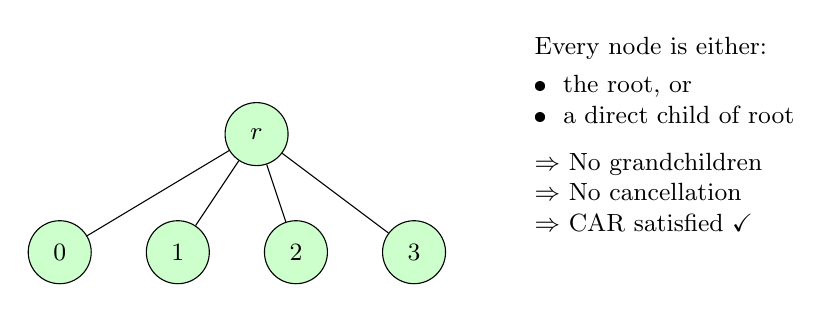
\begin{tikzpicture}[
  treeNode/.style={circle, draw, minimum size=0.8cm, inner sep=0pt,
                   font=\small},
  >=Stealth
]
  \node[treeNode, fill=green!20] (r) at (0,0) {$r$};
  \foreach \i/\x in {0/-2.5, 1/-1, 2/0.5, 3/2} {
    \node[treeNode, fill=green!20] (n\i) at (\x,-1.5) {$\i$};
    \draw (r) -- (n\i);
  }

  % Annotations
  \node[right=3cm of r, align=left, font=\small] {%
    Every node is either:\\[3pt]
    \textbullet\; the root, or\\
    \textbullet\; a direct child of root\\[6pt]
    $\Rightarrow$ No grandchildren\\
    $\Rightarrow$ No cancellation\\
    $\Rightarrow$ CAR satisfied \checkmark};
\end{tikzpicture}
\caption{Star trees have no depth-2 paths, so the failure mechanism
cannot trigger.}
\label{fig:star-safe}
\end{figure}

%%--------------------------------------------------------------------
\subsection{The exhaustive census}

To independently confirm the structural proof, we enumerate
\textbf{all} labelled rooted trees for small $n$ (via Pr\"ufer
sequences~\cite{prufer1918}) and check every anticommutator symbolically:

\begin{center}
\begin{tabular}{@{}rrrrl@{}}
\toprule
$n$ & Total trees & Pass CAR & Stars & Non-star survivors \\
\midrule
1 &       1 &   1 &   1 & 0 \\
2 &       2 &   2 &   2 & 0 \\
3 &       9 &   3 &   3 & 0 \\
4 &      64 &   4 &   4 & 0 \\
5 &     625 &   5 &   5 & 0 \\
\bottomrule
\end{tabular}
\end{center}

No ``accidental'' successes.  No exceptions.  The structural result is
sharp: exactly the $n$ star trees pass, every one of the $n^{n-1} - n$
non-star trees fails.

%%====================================================================
\section{How F\# Uncovered the Theorem}
\label{sec:fsharp}

This result was not found by pen-and-paper analysis.  It emerged from
building a \textbf{fully symbolic} encoding library in F\# and watching
it fail.

%%--------------------------------------------------------------------
\subsection{The FockMap library}

The FockMap library implements fermion-to-qubit encodings as pure
algebraic transformations --- no floating-point arithmetic, no
approximations.  Every coefficient is a Gaussian rational, every Pauli
product is tracked exactly.

The key design decisions that enabled the discovery:

\begin{enumerate}
  \item \textbf{Exact arithmetic.}  Coefficients are complex rationals
    ($\mathbb{Q}[i]$), not floating-point.  This means cancellation errors
    are impossible: if a term should be zero, it \emph{is} zero.

  \item \textbf{Parameterized construction.}  The encoding is defined
    by an \texttt{EncodingScheme} record --- three functions
    $U$, $P$, $\Occ{\cdot}$ --- and a single generic algorithm builds
    the Majorana operators:

\begin{fsharpcode}[F\# encoding scheme type]
type EncodingScheme =
  { Update     : int -> int -> Set<int>
    Parity     : int -> Set<int>
    Occupation : int -> Set<int> }

(* c Majorana: X on {j} U U(j), Z on P(j) *)
let cMajorana scheme j n =
  let u = scheme.Update j n
  let p = scheme.Parity j
  (j, X) :: setAssign X u @ setAssign Z p

(* d Majorana: Y on j, X on U(j),
   Z on (P(j) XOR Occ(j)) \ {j} *)
let dMajorana scheme j n =
  let u   = scheme.Update j n
  let p   = scheme.Parity j
  let occ = scheme.Occupation j
  let dZ  = symmetricDifference p occ |> Set.remove j
  (j, Y) :: setAssign X u @ setAssign Z dZ
\end{fsharpcode}

  \item \textbf{Automated CAR verification.}  A test harness
    symbolically computes every anticommutator
    $\acomm{c_i}{c_j}$, $\acomm{d_i}{d_j}$, and
    $\acomm{c_i}{d_j}$ and checks them against the expected values.

  \item \textbf{Tree-parameterized generation.}  Index sets can be
    derived from any labelled rooted tree via a generic function:

\begin{fsharpcode}[Deriving index sets from a tree]
let treeEncodingScheme tree =
  { Update     = fun j n -> ancestors tree j
    Parity     = fun j   -> remainder tree j
                             |> Set.union (children tree j)
    Occupation = fun j   -> descendants tree j
                             |> Set.add j }
\end{fsharpcode}
\end{enumerate}

%%--------------------------------------------------------------------
\subsection{The moment of discovery}

The development followed a natural path:

\begin{figure}[h]
\centering
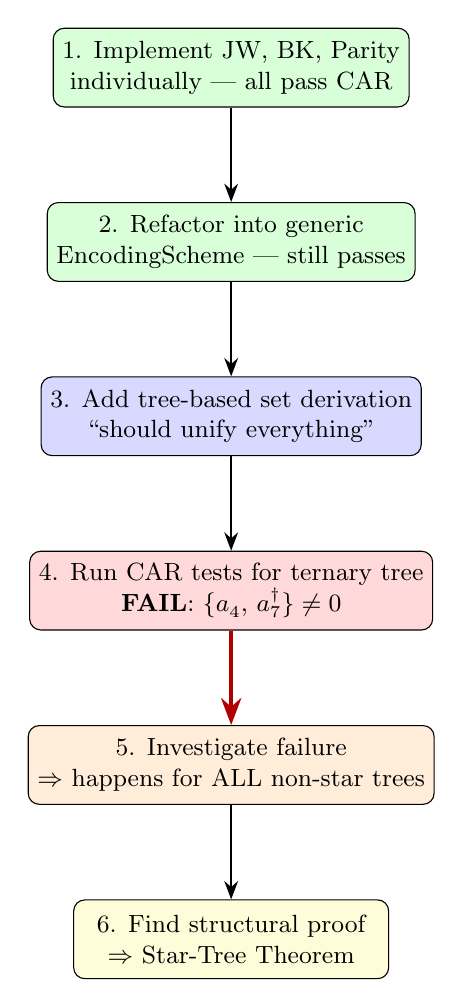
\begin{tikzpicture}[
  stepbox/.style={draw, rounded corners, minimum width=4cm,
               minimum height=1cm, align=center, font=\small},
  arr/.style={->, thick, >=Stealth},
  node distance=1.2cm
]
  \node[stepbox, fill=green!15] (s1)
    {1. Implement JW, BK, Parity\\individually --- all pass CAR};

  \node[stepbox, fill=green!15, below=of s1] (s2)
    {2. Refactor into generic\\EncodingScheme --- still passes};

  \node[stepbox, fill=blue!15, below=of s2] (s3)
    {3. Add tree-based set derivation\\``should unify everything''};

  \node[stepbox, fill=red!15, below=of s3] (s4)
    {4. Run CAR tests for ternary tree\\\textbf{FAIL}: $\acomm{\an{4}}{\ad{7}} \neq 0$};

  \node[stepbox, fill=orange!15, below=of s4] (s5)
    {5. Investigate failure\\$\Rightarrow$ happens for ALL non-star trees};

  \node[stepbox, fill=yellow!15, below=of s5] (s6)
    {6. Find structural proof\\$\Rightarrow$ Star-Tree Theorem};

  \draw[arr] (s1) -- (s2);
  \draw[arr] (s2) -- (s3);
  \draw[arr] (s3) -- (s4);
  \draw[arr, red!70!black, line width=1.5pt] (s4) -- (s5);
  \draw[arr] (s5) -- (s6);
\end{tikzpicture}
\caption{Timeline of discovery.  The critical moment (step~4) was
a test failure caused by the ternary tree's depth-2 structure.  The
exact symbolic computation left nowhere to hide.}
\label{fig:discovery-timeline}
\end{figure}

\begin{keyinsight}
The crucial role of exact symbolic computation: a floating-point
implementation might have missed this.  The spurious terms in the
anticommutator are small ($\pm 0.5$), and in a noisy numerical
computation they could be mistaken for rounding errors.  F\#'s
exact arithmetic made the failure unambiguous.
\end{keyinsight}

%%--------------------------------------------------------------------
\subsection{The diagnostic output}

When the ternary tree ($n = 8$) fails, the CAR test produces explicit
spurious terms.  For $\acomm{\an{4}}{\ad{7}}$, the computation yields:

\begin{center}
\begin{tabular}{@{}ll@{}}
\toprule
Expected & Actual \\
\midrule
$0$ & $(+0.5i)\; ZZZZZIXY$ \\
    & $(-0.5)\;\; ZZZZZIXX$ \\
\bottomrule
\end{tabular}
\end{center}

Two nonzero Pauli strings that should be zero.  Note position~5
(the parent node): it has $I$ --- the ``hole'' predicted by the
structural proof.

%%====================================================================
\section{The Three-Construction Landscape}
\label{sec:landscape}

The theorem reveals that the field's mental model has been conflating
three distinct constructions:

\begin{figure}[h]
\centering
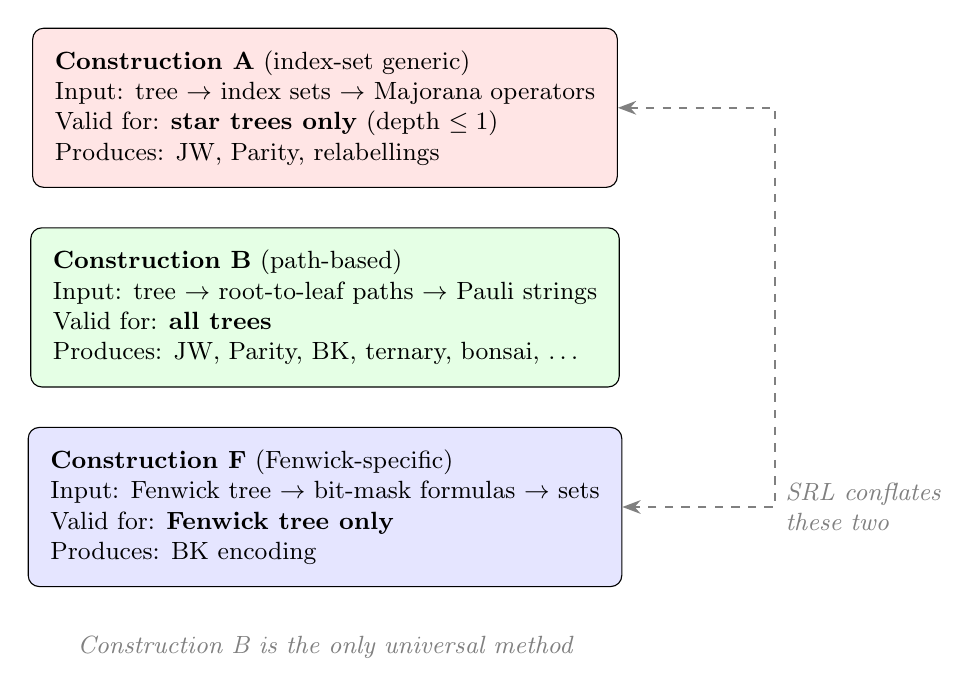
\begin{tikzpicture}[
  construct/.style={draw, rounded corners, minimum width=6cm,
                    minimum height=1.8cm, align=left, font=\small,
                    inner sep=8pt},
  >=Stealth
]
  % Construction A
  \node[construct, fill=red!10] (A) at (0,0)
    {\textbf{Construction A} (index-set generic)\\
     Input: tree $\to$ index sets $\to$ Majorana operators\\
     Valid for: \textbf{star trees only} (depth $\le 1$)\\
     Produces: JW, Parity, relabellings};

  % Construction B
  \node[construct, fill=green!10, below=0.5cm of A] (B)
    {\textbf{Construction B} (path-based)\\
     Input: tree $\to$ root-to-leaf paths $\to$ Pauli strings\\
     Valid for: \textbf{all trees}\\
     Produces: JW, Parity, BK, ternary, bonsai, \ldots};

  % Construction F
  \node[construct, fill=blue!10, below=0.5cm of B] (F)
    {\textbf{Construction F} (Fenwick-specific)\\
     Input: Fenwick tree $\to$ bit-mask formulas $\to$ sets\\
     Valid for: \textbf{Fenwick tree only}\\
     Produces: BK encoding};

  % Relationship annotations
  \draw[<->, thick, dashed, gray] (A.east) -- ++(2,0) |- (F.east)
    node[midway, right, font=\small\itshape, text=gray, align=left]
      {SRL conflates\\these two};

  % Universe annotation
  \node[below=0.5cm of F, font=\small\itshape, text=gray]
    {Construction B is the only universal method};
\end{tikzpicture}
\caption{Three distinct encoding constructions.  The SRL framework
conflates A~and~F.  Only Construction~B works for all trees.}
\label{fig:three-constructions}
\end{figure}

\subsection{What this means for the Bravyi--Kitaev encoding}

The BK encoding is not ``broken'' --- it produces a perfectly valid
encoding.  But its correctness comes from Construction~F (Fenwick-specific
bit-manipulation), not from Construction~A (generic SRL recipe).
If you apply the \emph{generic} tree-to-sets recipe to a Fenwick-shaped
tree, you get a \emph{different} set of index sets that fail the CAR.

\begin{figure}[h]
\centering
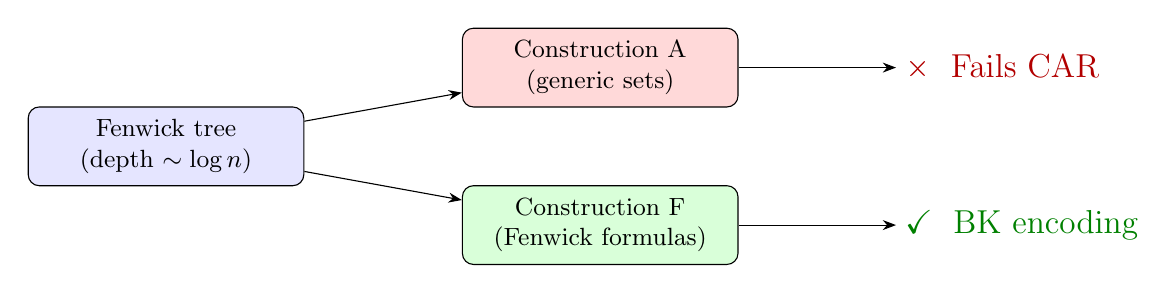
\begin{tikzpicture}[
  box/.style={draw, rounded corners, minimum width=3.5cm,
              minimum height=1cm, align=center, font=\small},
  >=Stealth
]
  \node[box, fill=blue!10] (fenwick) {Fenwick tree\\(depth $\sim \log n$)};

  \node[box, fill=red!15, right=2cm of fenwick, yshift=1cm] (consA)
    {Construction A\\(generic sets)};
  \node[box, fill=green!15, right=2cm of fenwick, yshift=-1cm] (consF)
    {Construction F\\(Fenwick formulas)};

  \node[right=2cm of consA, font=\large, text=red!70!black] (failX)
    {\texttimes\; Fails CAR};
  \node[right=2cm of consF, font=\large, text=green!50!black] (passC)
    {\checkmark\; BK encoding};

  \draw[->] (fenwick) -- (consA);
  \draw[->] (fenwick) -- (consF);
  \draw[->] (consA) -- (failX);
  \draw[->] (consF) -- (passC);
\end{tikzpicture}
\caption{The Fenwick tree produces different results depending on
which construction is applied.  The SRL paper uses Construction~F
(Fenwick-specific) but presents it as if it were Construction~A
(generic).}
\label{fig:fenwick-two-paths}
\end{figure}

%%====================================================================
\section{How the Fenwick Bit-Arithmetic Works (Construction F)}
\label{sec:construction-f}

The Bravyi--Kitaev encoding uses a deep tree (the Fenwick tree, depth
$\sim \log_2 n$), yet it produces a perfectly valid encoding.  How?
Because it does \emph{not} use the generic tree-to-sets recipe
(Construction~A).  Instead, it uses hand-derived bit-manipulation
formulas specific to the Fenwick tree's structure.

%%--------------------------------------------------------------------
\subsection{The Fenwick tree}

The Fenwick tree (also called a binary indexed tree) is a data
structure from computer science, originally designed for efficient
prefix-sum computation.  For $n$ nodes indexed $\{0, \ldots, n{-}1\}$,
the parent of node~$j$ is $j + \mathrm{lsb}(j)$, where
$\mathrm{lsb}(j) = j \mathbin{\&} (-j)$ is the least significant bit.

For $n = 8$:

\begin{figure}[h]
\centering
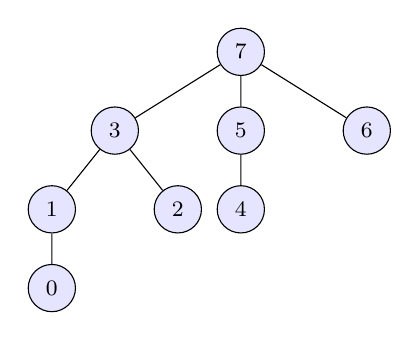
\begin{tikzpicture}[
  level distance=10mm, sibling distance=16mm,
  every node/.style={circle,draw,minimum size=6mm,inner sep=0pt,
    font=\footnotesize, fill=blue!10}
]
\node {7}
  child { node {3}
    child { node {1}
      child { node {0} }
    }
    child { node {2} }
  }
  child { node {5}
    child { node {4} }
  }
  child { node {6} };
\end{tikzpicture}
\caption{The Fenwick tree on 8 nodes.  Note the irregular, asymmetric
structure determined by binary representations of the indices.
This tree has depth~3.}
\label{fig:fenwick-tree}
\end{figure}

%%--------------------------------------------------------------------
\subsection{The bit-manipulation formulas}

Construction~F derives the three index sets using bit arithmetic, not
tree traversal:
\begin{align*}
  U_\text{BK}(j) &= \{j + \mathrm{lsb}(j),\;
    j + \mathrm{lsb}(j) + \mathrm{lsb}(j + \mathrm{lsb}(j)),\;
    \ldots\}, \\
  P_\text{BK}(j) &= \{j - 1,\;
    j - 1 - \mathrm{lsb}(j - 1),\; \ldots\}, \\
  \Occ{}_\text{BK}(j) &= \{j,\;
    j - \mathrm{lsb}(j),\; \ldots\}.
\end{align*}

These formulas produce $O(\log_2 n)$-sized sets, giving the
logarithmic Pauli weight that makes BK attractive.

%%--------------------------------------------------------------------
\subsection{Worked example: node 5 in the $n = 8$ Fenwick tree}

Let's compute the sets for $j = 5$ using both constructions:

\begin{center}
\begin{tabular}{@{}lcl@{}}
\toprule
& \textbf{Construction A} (generic) &
  \textbf{Construction F} (Fenwick bit formulas) \\
\midrule
$U(5)$ & $\{7\}$ (ancestors) &
  $\{6, 7\}$ ($5 + 1 = 6$, $6 + 2 = 8 > 7 \to$ stop at 7) \\
$P(5)$ & $\{4\} \cup \{3\}$ &
  $\{4\}$ ($5 - 1 = 4$, $\mathrm{lsb}(4) = 4 \to$ stop) \\
$\Occ{5}$ & $\{4, 5\}$ (descendants + self) &
  $\{5, 4\}$ ($5$, $5 - 1 = 4$, $\mathrm{lsb}(4) = 4 \to$ stop) \\
\bottomrule
\end{tabular}
\end{center}

Notice: the \textbf{update sets differ}.  Construction~A gives
$U(5) = \{7\}$ (just the ancestors in the tree), while Construction~F
gives $U(5) = \{6, 7\}$ (computed via bit arithmetic).  The parity
sets also differ.  These are \emph{different index sets} fed into the
same formula, producing \emph{different Pauli strings}.

\begin{keyinsight}
Construction~A and Construction~F, applied to the same tree shape,
produce \emph{different} index sets and therefore \emph{different}
operators.  Construction~F's operators satisfy the CAR;
Construction~A's do not.  The Fenwick tree is not a star, so the
star-tree theorem guarantees that Construction~A fails on it ---
and it does.
\end{keyinsight}

%%--------------------------------------------------------------------
\subsection{Why Construction F works}

The bit-manipulation formulas were hand-derived by Seeley, Richard,
and Love to ensure that the resulting index sets produce valid
encodings \emph{for the Fenwick tree specifically}.  They exploit the
unique algebraic properties of binary representations:
\begin{itemize}
  \item The update set uses $j + \mathrm{lsb}(j)$ to propagate
    changes through the prefix-sum structure --- this is \emph{not}
    the same as walking up ancestors in the tree.
  \item The parity set uses $j - 1$ and successive bit-stripping to
    collect the right parity information --- this is \emph{not} the
    remainder-plus-children formula of Construction~A.
  \item The occupation set similarly uses bit arithmetic rather than
    descendant enumeration.
\end{itemize}

These formulas happen to produce the right answer for the Fenwick
tree and no other tree.  There is no known way to generalise them.

%%--------------------------------------------------------------------
\subsection{The key takeaway}

\begin{center}
\begin{tabular}{@{}p{5.5cm}p{5.5cm}@{}}
\toprule
\textbf{Construction A} & \textbf{Construction F} \\
\midrule
Derive sets from tree structure\newline
(ancestors, remainder, descendants) &
Derive sets from bit arithmetic\newline
($\mathrm{lsb}$, $\mathbin{\&}$, shifts) \\
\addlinespace
General recipe: works for \emph{any} tree shape &
Specific recipe: works for \emph{Fenwick tree only} \\
\addlinespace
Produces valid encodings only for stars &
Produces a valid encoding (BK) \\
\addlinespace
Result: JW, Parity, relabellings &
Result: Bravyi--Kitaev only \\
\bottomrule
\end{tabular}
\end{center}

The SRL paper presents both JW/Parity (derived via A on star trees)
and BK (derived via F on the Fenwick tree) using the same notation,
giving the appearance that they come from the same construction.  They
do not.  BK is a \emph{Construction~F} instance wearing
Construction~A clothing.

%%====================================================================
\section{How Path-Based Encodings Work (Construction B)}
\label{sec:construction-b}

We have seen that Construction~A (the generic index-set recipe) fails
for all but star trees, and Construction~F only works for the Fenwick
tree.  So how do we encode fermions using \emph{arbitrary} trees?  The
answer is Construction~B: the \emph{path-based}
method introduced by Steudtner \& Wehner~\cite{steudtner2018} and
generalised by Jiang et al.~\cite{jiang2020} and Miller et
al.~\cite{miller2023bonsai}.

%%--------------------------------------------------------------------
\subsection{The idea in one sentence}

Instead of deriving index sets from a tree and feeding them into a
formula, read off Pauli operators \emph{directly} by walking from the
root to each leaf.

%%--------------------------------------------------------------------
\subsection{Encoding trees}

An \emph{encoding tree} is a rooted tree where:
\begin{itemize}
  \item Each internal node corresponds to one qubit.
  \item Each node has at most \textbf{three} descending connections
    (edges to children, or ``legs'' --- dangling terminal links).
  \item Each connection is labelled with a distinct Pauli:
    $X$, $Y$, or $Z$.
\end{itemize}

The branching limit of three comes directly from the Pauli algebra:
there are exactly three non-identity single-qubit operators, so a
node can have at most three outgoing links with distinct labels.

Fermionic modes are assigned to \emph{pairs} of legs.  Each mode~$j$
gets two legs $\ell_j^{(c)}$ and $\ell_j^{(d)}$, which will produce
the two Majorana operators $c_j$ and $d_j$.

%%--------------------------------------------------------------------
\subsection{Reading off Pauli strings}

To construct the Majorana operator for a leg $\ell$:
\begin{enumerate}
  \item Walk from the \textbf{root} to $\ell$.
  \item At each node on the path, place the \textbf{label} of the
    outgoing edge/leg on that qubit.
  \item At every node \textbf{not} on the path, place identity~$I$.
\end{enumerate}

That's it.  The Pauli string is the tensor product of all these
assignments.

%%--------------------------------------------------------------------
\subsection{Worked example: a ternary tree on 3 modes}

Consider a single root node with three outgoing legs labelled
$X$, $Y$, $Z$.  We pair them into one mode and add a child:

\begin{figure}[h]
\centering
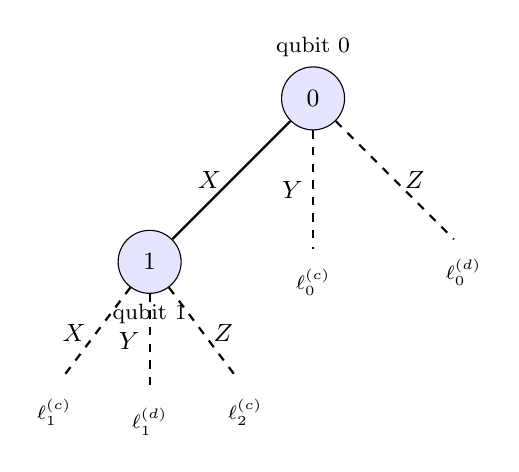
\begin{tikzpicture}[
  node distance=1.5cm,
  treeNode/.style={circle, draw, fill=blue!10, minimum size=0.8cm,
                   inner sep=0pt, font=\small},
  leg/.style={thick, dashed},
  lbl/.style={font=\small\bfseries, midway},
  >=Stealth
]
  % Root (qubit 0)
  \node[treeNode, label={[font=\footnotesize]above:qubit 0}] (root) {0};

  % Three connections from root
  \node[treeNode, label={[font=\footnotesize]below:qubit 1},
        below left=1.5cm and 1.5cm of root] (child) {1};
  \node[below=1.5cm of root] (leg_y) {};
  \node[below right=1.5cm and 1.5cm of root] (leg_z) {};

  % Edge to child
  \draw[thick] (root) -- node[lbl, left] {$X$} (child);

  % Legs from root
  \draw[leg] (root) -- node[lbl, left] {$Y$} (leg_y)
    node[below, font=\scriptsize] {$\ell_0^{(c)}$};
  \draw[leg] (root) -- node[lbl, right] {$Z$} (leg_z)
    node[below, font=\scriptsize] {$\ell_0^{(d)}$};

  % Legs from child
  \node[below left=1.2cm and 0.8cm of child] (c_leg1) {};
  \node[below=1.2cm of child] (c_leg2) {};
  \node[below right=1.2cm and 0.8cm of child] (c_leg3) {};

  \draw[leg] (child) -- node[lbl, left] {$X$} (c_leg1)
    node[below, font=\scriptsize] {$\ell_1^{(c)}$};
  \draw[leg] (child) -- node[lbl, left] {$Y$} (c_leg2)
    node[below, font=\scriptsize] {$\ell_1^{(d)}$};
  \draw[leg] (child) -- node[lbl, right] {$Z$} (c_leg3)
    node[below, font=\scriptsize] {$\ell_2^{(c)}$};

  % Mode 2's second leg would come from elsewhere, skip for clarity
\end{tikzpicture}
\caption{A small encoding tree with 2 qubits (nodes 0 and 1) and
5 legs.  Dashed lines are legs; the solid line is an edge.
Legs are paired into modes: mode~0 gets $\ell_0^{(c)}$ and
$\ell_0^{(d)}$; mode~1 gets $\ell_1^{(c)}$ and $\ell_1^{(d)}$.}
\label{fig:encoding-tree-example}
\end{figure}

Reading off the Pauli strings:

\begin{center}
\begin{tabular}{@{}llll@{}}
\toprule
Operator & Path & Qubit 0 & Qubit 1 \\
\midrule
$c_0 = S(\ell_0^{(c)})$ & root $\xrightarrow{Y}$ leg
  & $Y$ & $I$ \\
$d_0 = S(\ell_0^{(d)})$ & root $\xrightarrow{Z}$ leg
  & $Z$ & $I$ \\
$c_1 = S(\ell_1^{(c)})$ & root $\xrightarrow{X}$ node\,1 $\xrightarrow{X}$ leg
  & $X$ & $X$ \\
$d_1 = S(\ell_1^{(d)})$ & root $\xrightarrow{X}$ node\,1 $\xrightarrow{Y}$ leg
  & $X$ & $Y$ \\
\bottomrule
\end{tabular}
\end{center}

So: $c_0 = Y \otimes I$, \; $d_0 = Z \otimes I$, \;
$c_1 = X \otimes X$, \; $d_1 = X \otimes Y$.

%%--------------------------------------------------------------------
\subsection{Why does it always work?}

The correctness proof is beautifully simple.  Take any two Majorana
operators $S(\ell_a)$ and $S(\ell_b)$ from different legs:

\begin{enumerate}
  \item Their root-to-leg paths share a \textbf{common prefix} (they
    start at the same root).
  \item At some node, they \textbf{diverge}: $\ell_a$'s path takes one
    child (label $\sigma_a$) and $\ell_b$'s path takes another
    (label $\sigma_b$), with $\sigma_a \neq \sigma_b$.
  \item At the divergence node: $\sigma_a \sigma_b = -\sigma_b
    \sigma_a$ (distinct Paulis anticommute).
  \item On the shared prefix: same labels $\to$ they commute.
  \item Below the divergence: one operator has identity where the
    other is non-trivial $\to$ they commute.
\end{enumerate}

Total anticommuting positions: exactly \textbf{one} (the divergence
node).  One is odd, so $\{S(\ell_a), S(\ell_b)\} = 0$.  \checkmark

\begin{keyinsight}
Construction~B works because distinct paths through a branching tree
\emph{necessarily} anticommute at exactly one node --- the point where
they diverge.  No constraints on tree shape, depth, or labelling are
needed.  The tree structure \emph{is} the proof.
\end{keyinsight}

%%--------------------------------------------------------------------
\subsection{Verification on our example}

Let's check: $\{c_0, c_1\} = \{Y \otimes I,\; X \otimes X\}$.

Position~0: $Y \cdot X = -X \cdot Y$ (anticommutes).
Position~1: $I \cdot X = X \cdot I$ (commutes).
Total anticommuting: 1 (odd).  So $\{c_0, c_1\} = 0$. \checkmark

And $\{c_1, d_1\} = \{X \otimes X,\; X \otimes Y\}$.

Position~0: $X \cdot X = I$ (commutes).
Position~1: $X \cdot Y = -Y \cdot X$ (anticommutes).
Total: 1 (odd).  So $\{c_1, d_1\} = 0$. \checkmark

Every pair works, for any tree.  That's the power of the path-based
approach.

%%--------------------------------------------------------------------
\subsection{Contrast with Construction A}

Why does Construction~A fail where Construction~B succeeds?
The difference is conceptual:

\begin{center}
\begin{tabular}{@{}p{5.5cm}p{5.5cm}@{}}
\toprule
\textbf{Construction A (index-set)} & \textbf{Construction B (path-based)} \\
\midrule
Derives sets $U$, $P$, $\mathrm{Occ}$ from the tree &
Reads Pauli labels directly from tree paths \\
\addlinespace
Applies a universal formula to the sets &
No formula --- the path \emph{is} the operator \\
\addlinespace
Sets can overlap and cancel (symmetric difference) &
No cancellation possible \\
\addlinespace
The cancellation creates identity at positions that should
anticommute (the ``even count'' failure) &
Every divergence produces exactly one anticommuting position \\
\addlinespace
Works only for stars &
Works for all trees \\
\bottomrule
\end{tabular}
\end{center}

The root cause of Construction~A's failure (recall
\cref{fig:failure-mechanism}): on a grandparent--parent--grandchild
path $w \to u \to v$, node~$u$ appears in both $P(w)$ and
$\mathrm{Occ}(w)$, so it cancels in the symmetric difference.  This
gives $d_w$ identity at position~$u$, where $c_v$ has a non-identity
Pauli.  The result: \emph{two} anticommuting positions (even) instead
of one (odd).

Construction~B avoids this entirely.  There is no symmetric difference,
no set arithmetic, no possibility of cancellation.  The Pauli
assignment comes straight from the tree, position by position.

%%--------------------------------------------------------------------
\subsection{Recovering standard encodings}

All five standard encodings emerge from specific tree topologies:

\begin{center}
\begin{tabular}{@{}llc@{}}
\toprule
Tree shape & Encoding & Max weight \\
\midrule
Star (1 root, $n$ legs) & Jordan--Wigner & $O(n)$ \\
Star (reversed labelling) & Parity & $O(n)$ \\
Fenwick tree & Bravyi--Kitaev & $O(\log_2 n)$ \\
Balanced binary tree & Binary tree & $O(\log_2 n)$ \\
Balanced ternary tree & Ternary tree & $O(\log_3 n)$ \\
\bottomrule
\end{tabular}
\end{center}

The weight bound is $O(\text{depth of tree})$.  Shallower trees (stars)
have high weight because the single root participates in every
operator.  Deeper, balanced trees distribute the work and achieve
logarithmic weight.

The balanced ternary tree achieves the \emph{optimal} Pauli weight
among all tree-based encodings: it uses all three non-identity Paulis
at every node, maximising branching and minimising depth.

%%====================================================================
\section{The $n^{n-1}$ Tree Landscape}
\label{sec:counting}

By Cayley's formula, there are $n^{n-1}$ labelled rooted trees on
$[n]$ vertices.  The star-tree theorem partitions this space cleanly:

\begin{figure}[h]
\centering
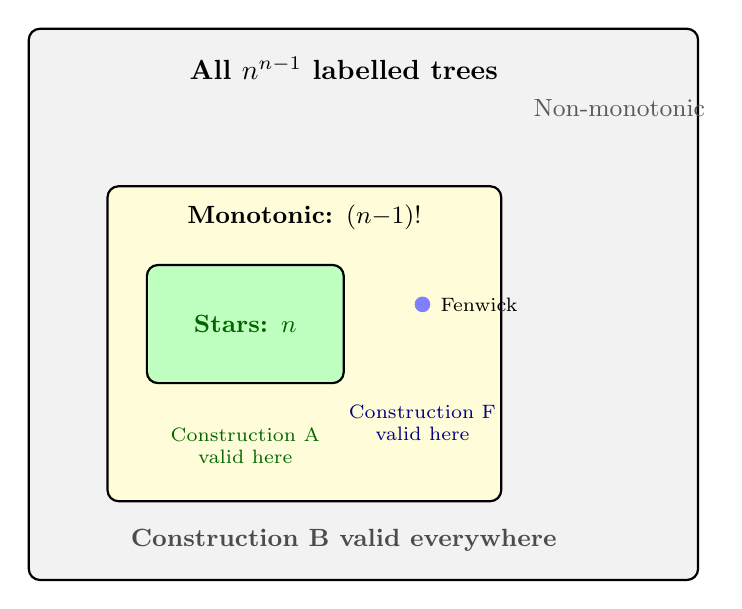
\begin{tikzpicture}[
  >=Stealth
]
  % Universe
  \draw[thick, fill=gray!10, rounded corners]
    (-4,-3.5) rectangle (4.5,3.5);
  \node[font=\bfseries] at (0,3) {All $n^{n-1}$ labelled trees};

  % Monotonic region
  \draw[thick, fill=yellow!15, rounded corners]
    (-3,-2.5) rectangle (2,1.5);
  \node[font=\small\bfseries] at (-0.5,1.1) {Monotonic: $(n{-}1)!$};

  % Star region (inside monotonic)
  \draw[thick, fill=green!25, rounded corners]
    (-2.5,-1) rectangle (0,0.5);
  \node[font=\small\bfseries, text=green!40!black] at (-1.25,-0.25)
    {Stars: $n$};

  % Fenwick point (inside monotonic, outside star)
  \node[circle, fill=blue!50, inner sep=2pt, label={[font=\scriptsize]right:Fenwick}]
    at (1,0) {};

  % Non-monotonic region
  \node[font=\small, text=gray!70!black] at (3.5,2.5)
    {Non-monotonic};

  % Construction labels
  \node[font=\scriptsize, text=green!40!black, align=center] at (-1.25,-1.8)
    {Construction A\\valid here};
  \node[font=\scriptsize, text=blue!50!black, align=center] at (1,-1.5)
    {Construction F\\valid here};

  % Construction B annotation
  \node[font=\small\bfseries, text=gray!60!black] at (0,-3)
    {Construction B valid \textbf{everywhere}};
\end{tikzpicture}
\caption{The space of labelled rooted trees, showing regions where
each construction is valid.  Stars are a vanishing fraction of all
trees; Construction~B is the only universal method.}
\label{fig:tree-landscape}
\end{figure}

\begin{center}
\begin{tabular}{@{}rlll@{}}
\toprule
$n$ & Total trees & Monotonic & Stars \\
\midrule
3 &       9 &    2 (22\%) &   3 (33\%) \\
4 &      64 &    6 (9\%) &   4 (6\%) \\
5 &     625 &   24 (4\%) &   5 (0.8\%) \\
8 & 2,097,152 & 5,040 (0.24\%) & 8 (0.0004\%) \\
\bottomrule
\end{tabular}
\end{center}

Stars represent a \emph{vanishing fraction} of all trees.  The SRL
framework's generic construction covers less than $n/n^{n-1} = 1/n^{n-2}$
of the design space.

%%====================================================================
\section{What Changes}
\label{sec:consequences}

\subsection{For encoding design}

\begin{itemize}
  \item \textbf{The path-based construction is king.}  If you want to
    try a new tree topology, use Construction~B (follow root-to-leaf
    paths), not Construction~A (derive index sets).  Construction~B is
    the only method that works for every tree.

  \item \textbf{Optimal encodings are unreachable by index sets.}  The
    balanced ternary tree (optimal $O(\log_3 n)$ weight) requires
    Construction~B.  There is no index-set derivation that produces it.

  \item \textbf{The BK encoding is more special than we thought.}  Its
    success is not evidence for the general index-set approach; it's a
    happy coincidence of Fenwick-tree number theory.
\end{itemize}

\subsection{For the literature}

\begin{itemize}
  \item Papers that cite SRL as a ``unified framework'' should qualify
    the claim: the framework unifies JW and Parity (both star-based)
    and happen to also express BK via a separate construction, but it
    does not generalize to arbitrary trees.

  \item The question ``which trees give good encodings?'' was being
    asked in the wrong construction.  In Construction~B, \emph{all}
    trees give valid encodings; the question is purely about weight
    optimization.
\end{itemize}

\subsection{For implementation}

\begin{itemize}
  \item Do not blindly implement the SRL formulas for arbitrary trees.
    Always verify CAR symbolically, or use the path-based method.

  \item The FockMap library provides both constructions and an
    automated CAR verification suite (497 tests), making it safe
    to explore novel tree topologies.
\end{itemize}

%%====================================================================
\section{Summary}
\label{sec:summary}

\begin{figure}[h]
\centering
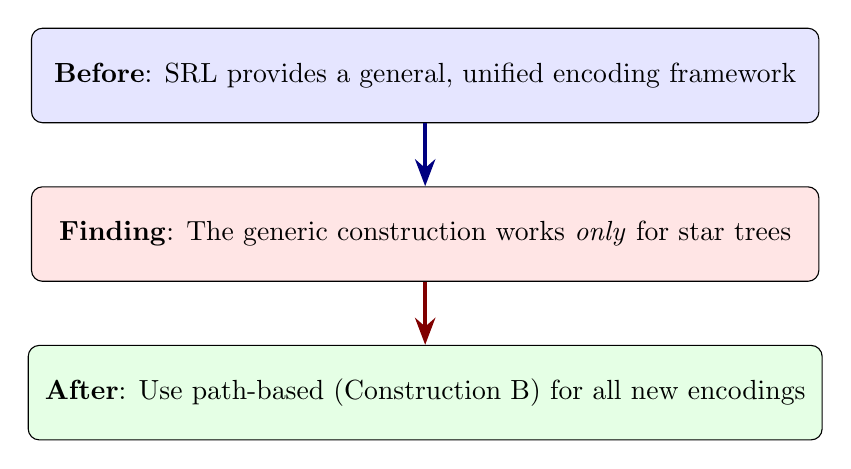
\begin{tikzpicture}[
  box/.style={draw, rounded corners, minimum width=10cm,
              minimum height=1.2cm, align=center, font=\normalsize,
              inner sep=6pt},
  arr/.style={->, thick, >=Stealth, line width=1.5pt},
  node distance=0.8cm
]
  \node[box, fill=blue!10] (before)
    {\textbf{Before}: SRL provides a general, unified encoding framework};

  \node[box, fill=red!10, below=of before] (find)
    {\textbf{Finding}: The generic construction works \emph{only} for
     star trees};

  \node[box, fill=green!10, below=of find] (after)
    {\textbf{After}: Use path-based (Construction~B) for all new
     encodings};

  \draw[arr, blue!50!black] (before) -- (find);
  \draw[arr, red!50!black] (find) -- (after);
\end{tikzpicture}
\caption{The star-tree theorem in one slide.}
\label{fig:one-slide}
\end{figure}

The star-tree theorem reveals a structural limitation hiding in plain
sight.  The SRL index-set framework, while elegant, is far less general
than commonly assumed.  The proof is elementary (count anticommuting
positions on a three-vertex path), the implication is significant
(most of the encoding design space requires a different construction),
and the discovery was enabled by exact symbolic computation in F\#.

\bigskip

\noindent\textbf{Code availability.}
The FockMap library, including all verification tests, is open source
at \url{https://github.com/johnazariah/encodings}.

%%====================================================================
\section{Literature Review: Has This Been Found Before?}
\label{sec:prior-work}

A natural question: is the star-tree limitation already known?  We
surveyed the core fermion-to-qubit encoding literature systematically.
The answer is \textbf{no} --- no published paper proves, states, or
hints at this result.

%%--------------------------------------------------------------------
\subsection{Papers that define or use the SRL framework}

\begin{description}[leftmargin=1.5cm]
  \item[Seeley, Richard \& Love (2012)~\cite{seeley2012}.]
    The originating paper.  Presents the index-set framework for JW,
    BK, and Parity.  Demonstrates that all three can be expressed as
    triples $(U, P, \mathrm{Occ})$ fed into a single algorithm.  Does
    \emph{not} prove the algorithm works for arbitrary index sets or
    arbitrary trees.  Does \emph{not} warn that it might fail.  The
    paper's presentation naturally suggests generality, and subsequent
    work has treated it as such.

    \textbf{Key gap:} The paper conflates two constructions --- the
    generic algorithm (our Construction~A) and the Fenwick-specific
    derivation for BK (our Construction~F) --- without distinguishing
    them.

  \item[Tranter et al.\ (2015)~\cite{tranter2015}.]
    Comparative study of JW and BK for molecular simulation.  Builds
    on the SRL framework without questioning its generality.  Does not
    attempt to apply the framework to non-standard trees.

  \item[Havl\'{i}\v{c}ek, Troyer \& Whitfield (2017)~\cite{havlicek2017}.]
    Proves operator-theoretic lower bounds on encoding overhead.  Does
    not analyze the SRL construction's domain of validity.  Treats the
    index-set framework as a given.
\end{description}

%%--------------------------------------------------------------------
\subsection{Papers that introduce alternative constructions}

\begin{description}[leftmargin=1.5cm]
  \item[Steudtner \& Wehner (2018)~\cite{steudtner2018}.]
    Introduces a ternary-tree-based unifying framework and proves
    $O(\log_3 n)$ Pauli-weight bounds.  Their construction is
    \emph{path-based} (our Construction~B): Majorana operators are
    built by collecting Pauli labels along root-to-leaf paths, not by
    deriving index sets.

    \textbf{Relationship to our result:} Steudtner \& Wehner's work
    is complementary.  They provide the universal construction that
    \emph{does} work for all trees, but they do not explain \emph{why}
    the index-set alternative fails.  The star-tree theorem provides a
    retroactive explanation: the path-based construction was necessary
    because the index-set construction is valid only for stars.

  \item[Jiang et al.\ (2020)~\cite{jiang2020}.]
    Introduces path-based encodings for ternary trees with optimal
    weight scaling.  Like Steudtner \& Wehner, uses Construction~B.
    Does not discuss limitations of the index-set (Construction~A)
    approach.  Simply presents path-based encoding as a new method
    without noting that the older method fails for the same trees.

  \item[Miller et al.\ (2023, Bonsai)~\cite{miller2023bonsai}.]
    Generalizes path-based encodings to arbitrary tree topologies
    (``bonsai'' trees).  Again uses Construction~B.  Does not identify
    the failure of Construction~A for non-star trees.  The implicit
    assumption appears to be that path-based and index-set methods
    are simply two valid alternatives.
\end{description}

%%--------------------------------------------------------------------
\subsection{Papers on related but distinct topics}

\begin{description}[leftmargin=1.5cm]
  \item[Bravyi \& Kitaev (2002)~\cite{bravyi2002}.]
    Original BK encoding.  Uses Fenwick-tree bit manipulations directly
    (Construction~F).  Does not use the SRL framework (which came a
    decade later).

  \item[Derby \& Klassen (2021)~\cite{derby2021}.]
    Compact fermion-to-qubit mappings using auxiliary qubits.  Operates
    in a different domain (qubit-saving encodings with ancillae) and
    does not discuss the SRL framework's limitations.

  \item[Bravyi et al.\ (2017)~\cite{bravyi2017tapering}.]
    Tapering off qubits using symmetries.  Orthogonal to the
    construction-validity question.
\end{description}

%%--------------------------------------------------------------------
\subsection{Summary of literature findings}

\begin{center}
\begin{tabular}{@{}p{4cm}ccc@{}}
\toprule
Paper & \parbox{2cm}{\centering Uses\\Construction} &
  \parbox{2.2cm}{\centering Identifies\\A/B/F split?} &
  \parbox{2.2cm}{\centering Proves star\\limitation?} \\
\midrule
SRL (2012) & A + F & No & No \\
Tranter (2015) & A (via SRL) & No & No \\
Havl\'{i}\v{c}ek (2017) & --- & No & No \\
Steudtner \& Wehner (2018) & B & No & No \\
Jiang (2020) & B & No & No \\
Miller / Bonsai (2023) & B & No & No \\
Bravyi \& Kitaev (2002) & F & No & No \\
Derby \& Klassen (2021) & --- & No & No \\
\midrule
\textbf{This work} & \textbf{A, B, F} & \textbf{Yes} & \textbf{Yes} \\
\bottomrule
\end{tabular}
\end{center}

\begin{keyinsight}
The literature splits cleanly into two groups: (1)~papers that use the
SRL index-set framework without questioning its generality, and
(2)~papers that introduce path-based alternatives without explaining
why they were needed.  No paper bridges the gap by identifying the
structural failure of the index-set approach.  The star-tree theorem
fills this gap.
\end{keyinsight}

%%====================================================================
%% Appendix
%%====================================================================
\appendix

\section{The Original: How Jordan--Wigner Works (1928)}
\label{app:jordan-wigner}

Every encoding in this document descends, directly or indirectly, from
the transformation that Pascual Jordan and Eugene Wigner published in
1928~\cite{jordan1928}.  Their paper, ``\"{U}ber das Paulische
\"{A}quivalenzverbot'' (On the Pauli exclusion principle), introduced
the idea that would eventually make quantum chemistry on quantum
computers possible.  For completeness --- and to give proper credit
to the OGs --- we present the construction in modern notation.

\subsection*{The problem}

Fermions are particles that obey the Pauli exclusion principle: no two
can occupy the same quantum state.  Mathematically, this is encoded in
the \emph{canonical anticommutation relations} (CAR):
\begin{align}
  \acomm{\an{i}}{\ad{j}} &= \delta_{ij}, \\
  \acomm{\an{i}}{\an{j}} &= 0, \\
  \acomm{\ad{i}}{\ad{j}} &= 0.
\end{align}

Qubits, on the other hand, are distinguishable two-level systems
that naturally \emph{commute} across different sites.  The challenge
is: how do you represent anticommuting particles using commuting
degrees of freedom?

\subsection*{Jordan and Wigner's insight}

The key idea is a \emph{parity string}.  For each fermionic mode~$j$,
attach a chain of $Z$ operators on all lower-index qubits to enforce
the sign change:
\begin{align}
  \ad{j} &= \tfrac{1}{2}(X_j - iY_j) \otimes
    Z_{j-1} \otimes Z_{j-2} \otimes \cdots \otimes Z_0, \\
  \an{j} &= \tfrac{1}{2}(X_j + iY_j) \otimes
    Z_{j-1} \otimes Z_{j-2} \otimes \cdots \otimes Z_0.
\end{align}

In the Majorana language that we use throughout this document:
\begin{align}
  c_j &= X_j \otimes Z_{j-1} \otimes \cdots \otimes Z_0, \\
  d_j &= Y_j \otimes Z_{j-1} \otimes \cdots \otimes Z_0.
\end{align}

The $Z$ string ``remembers'' the parity of all occupied modes below
index~$j$.  Since $Z\ket{0} = +\ket{0}$ and $Z\ket{1} = -\ket{1}$,
every occupied mode below~$j$ contributes a minus sign, producing
exactly the sign flip that anticommutation requires.

\subsection*{Worked example: $n = 4$ modes}

\begin{center}
\begin{tabular}{@{}cll@{}}
\toprule
Mode $j$ & $c_j$ & $d_j$ \\
\midrule
0 & $X \otimes I \otimes I \otimes I$ &
    $Y \otimes I \otimes I \otimes I$ \\
1 & $Z \otimes X \otimes I \otimes I$ &
    $Z \otimes Y \otimes I \otimes I$ \\
2 & $Z \otimes Z \otimes X \otimes I$ &
    $Z \otimes Z \otimes Y \otimes I$ \\
3 & $Z \otimes Z \otimes Z \otimes X$ &
    $Z \otimes Z \otimes Z \otimes Y$ \\
\bottomrule
\end{tabular}
\end{center}

The pattern is unmistakable: qubit~$j$ gets the ``active'' Pauli
($X$ for $c_j$, $Y$ for $d_j$), qubits $0$ through $j{-}1$ each
get~$Z$, and qubits above~$j$ get identity.

\subsection*{Why it works: verifying the CAR}

Consider $c_1 = ZXII$ and $c_2 = ZZXI$.  Multiplying
position-by-position:
\begin{align*}
  c_1 \cdot c_2 &: \quad
    \underbrace{Z \cdot Z}_{+I} \;\otimes\;
    \underbrace{X \cdot Z}_{-iY} \;\otimes\;
    \underbrace{I \cdot X}_{+X} \;\otimes\;
    \underbrace{I \cdot I}_{+I}, \\
  c_2 \cdot c_1 &: \quad
    \underbrace{Z \cdot Z}_{+I} \;\otimes\;
    \underbrace{Z \cdot X}_{+iY} \;\otimes\;
    \underbrace{X \cdot I}_{+X} \;\otimes\;
    \underbrace{I \cdot I}_{+I}.
\end{align*}

At position~1, $XZ = -ZX$ --- this is the only position where the two
operators differ in a non-trivial way.  One anticommuting position
(odd count) means $\acomm{c_1}{c_2} = 0$. \checkmark

For same-mode: $c_1 \cdot c_1 = I^{\otimes 4}$ since $Z^2 = X^2 = I$,
so $\acomm{c_1}{c_1} = 2I$. \checkmark

The argument generalises: for any $i < j$, the operators $c_i$ and
$c_j$ share $Z$ strings on qubits $0, \ldots, i{-}1$ (which commute
when squared), differ at qubit~$i$ where $c_i$ has $X$ and $c_j$
has~$Z$ ($XZ = -ZX$, one anticommuting position), and have
non-overlapping support above qubit~$i$.  The result is always
exactly one anticommuting position, so distinct Majoranas always
anticommute.

\subsection*{The cost}

The Pauli weight of $c_j$ (and $d_j$) is $j + 1$: one $X$ or $Y$
plus $j$ copies of $Z$.  For the highest mode, the weight is~$n$.

For a molecular Hamiltonian with 100 spin-orbitals, a hopping term
$\ad{0}\an{99}$ becomes a 100-qubit Pauli string.  This $O(n)$
scaling is what motivated the entire field of alternative encodings ---
and everything else in this document.

\subsection*{Historical context}

Jordan and Wigner's 1928 paper was not about quantum computing
(which wouldn't be conceived for another 50+ years).  They were
studying the equivalence between certain spin-chain models and
fermionic systems in condensed-matter physics.  The transformation
showed that a chain of interacting spins could be re-interpreted as a
system of non-interacting fermions, and vice versa --- a duality that
remains central to condensed-matter theory.

It was Aspuru-Guzik et al.~\cite{aspuruguzik2005} who, in 2005,
first used the Jordan--Wigner transformation as a step in a quantum
algorithm for chemistry, turning a mathematical curiosity from 1928
into a practical tool for quantum simulation.  Whitfield, Biamonte, and
Aspuru-Guzik~\cite{whitfield2011} then codified the full pipeline
(molecular integrals $\to$ second quantization $\to$ JW $\to$ Pauli
Hamiltonian) that remains the standard workflow today.

Nearly a century after its invention, Jordan--Wigner is still the
default encoding in every major quantum computing framework --- and
the benchmark against which every subsequent encoding is measured.

%%====================================================================
\bibliography{../shared/bibliography/references}
\bibliographystyle{plain}

\end{document}
